\documentclass[]{statsoc}
\usepackage{enumitem}
\usepackage{natbib}
\usepackage{setspace}
\usepackage{geometry}                % See geometry.pdf to learn the layout options. There are lots.
\geometry{letterpaper}                   % ... or a4paper or a5paper or ... 
%\geometry{landscape}                % Activate for for rotated page geometry
%\usepackage[parfill]{parskip}    % Activate to begin paragraphs with an empty line rather than an indent
\usepackage{graphicx}
\usepackage{amssymb}
\usepackage{amsmath}
\usepackage{epstopdf}
\usepackage[linesnumbered,vlined,algoruled]{algorithm2e}
\usepackage{url}
\usepackage{mathtools}
\DeclarePairedDelimiter{\ceil}{\lceil}{\rceil}
\DeclarePairedDelimiter{\floor}{\lfloor}{\rfloor}
\DeclareMathOperator*{\argmax}{arg\,max}
\DeclareMathOperator{\argmin}{arg\,min}
\setlength{\parskip}{0.5 em}

\title[Figure construction]{Figure construction for $t$-digest}

\author{Ted Dunning}
\date{}                                           % Activate to display a given date or no date
\begin{document}
\begin{abstract}
This short paper describes how to recreate the figures in the larger article
\end{abstract}
\maketitle
\section{Introduction}
The figures in the $t$-digest paper are generated using a variety of Java test cases, R scripts and hand-drawn figures. To regenerate these figures generally requires that you run the Java test cases to produce data that is reduced by R and then plotted in pdf form.

This document describes how to replicate all of the figures. The figures are included at the end of this document for reference together with their original captions.

Note that all figures must be moved to the {\tt docs/t-digest-paper/figures} directory to be available when formatting the paper.
\section{Figure \ref{fig:k-q-plot}}
Figure \ref{fig:k-q-plot} includes {\tt k-q-plot.pdf} which is produced by {\tt ./docs/t-digest-paper/k-q-plot.r }without using any external data.
\section{Figure \ref{fig:linear-interpolation}}
Figure \ref{fig:linear-interpolation} is based on {\tt linear-interpolation.pdf} which is produced by the R script {\tt linear-interpolation.r} found in {\tt ./docs/t-digest-paper/}. No external data is read by this script, but the sizes of the clusters on line 46 were taken from an actual $t$-digest.

\section{Figures \ref{fig:interpolation}, \ref{fig:singletons} and \ref{fig:endpoint}}
Figures \ref{fig:interpolation}, \ref{fig:singletons} and \ref{fig:endpoint} were all hand-drawn in Omnigraffle. The source for all of them is in {\tt quantile-figures.graffle}. Figure \ref{fig:interpolation} is found on canvas 5, Figure \ref{fig:singletons} is on canvas 4 and Figure \ref{fig:endpoint} is on canvas 6. To recreate the figures themselves, use File $>$ Export to bring up a dialog that will write all artboards to separate PDF files. The  \LaTeX source code assumes that these figures will be in the directory {\tt figures} and that directory has to be set during the export process.
\section{Figure \ref{fig:by-scale}}
Figure \ref{fig:by-scale} illustrates error rates for different scale functions and values of $q$. Production of the two graphs in this figure requires a series of steps to first generate the data in question and then to process and plot the data. Note that this figure will vary a fair bit each time you generate new data. This is due to the fact that the number of iterations used to generate the data is pretty small in order to keep the time required for the test to a reasonable level.

The data is generated by {\tt AccuracyTest.testAccuracyVersusCompression()} in the {\tt quality} module. The data is written to the directory {\tt quality/tests} with a pathname composed using the ``experiment'' and the git hash of the current version of the code. This structure allows you (and me) to generate the same figure for different versions of the code.

To generate this figure, you need to do the following steps:
\begin{enumerate}
\item In the {\tt quality} sub-directory, run {\tt AccuracyTest.testAccuracyVersusCompression}. This will produce a lot of measurements into {\tt quality/tests} and should take a few minutes. Note that running {\em all} of the tests in {\tt quality} will take tens of minutes.
\item look at the most recently generated files in {\tt quality/tests} to find out the current git hash. As an example, here is an extract of what I just saw when doing this
\begin{verbatim}
$ cd quality
$ ls -rt tests
    ...
accuracy-tree-digest-76e0eb8670.csv
accuracy-sizes-tree-digest-76e0eb8670.csv
accuracy-cdf-tree-digest-76e0eb8670.csv
accuracy-sizes-digest-a09d38d1d1.csv
accuracy-cdf-digest-a09d38d1d1.csv
accuracy-digest-a09d38d1d1.csv
\end{verbatim}
From this, I know that my current tag is {\tt a09d38d1d1}.
\item in R, read this data and plot it. To read the data, we specify an experiment (digest, in this case) and git hash which we learned in the previous step.
\begin{verbatim}
$ cd quality
$ R

R version 3.5.2 (2018-12-20) -- "Eggshell Igloo"
Copyright (C) 2018 The R Foundation for Statistical Computing
     ...
Type 'q()' to quit R.

> source('accuracy.r')
> read.data('digest', 'a09d38d1d1')
> draw.relative.error.fig()
foo MergingDigest-K_1-weight-alternating-twoLevel UNIFORM unsorted 100 NA 
624 10 
foo MergingDigest-K_2-weight-alternating-twoLevel UNIFORM unsorted 100 NA 
650 10 
foo MergingDigest-K_3-weight-alternating-twoLevel UNIFORM unsorted 100 NA 
624 10 
foo MergingDigest-K_1-weight-alternating-twoLevel UNIFORM unsorted 100 NA 
624 10 
foo MergingDigest-K_2-weight-alternating-twoLevel UNIFORM unsorted 100 NA 
650 10 
foo MergingDigest-K_3-weight-alternating-twoLevel UNIFORM unsorted 100 NA 
624 10 
null device 
          1 
> q()
Save workspace image? [y/n/c]: n
$ 
\end{verbatim}
This should generate {\tt relative-error.pdf} which can by copied to {\tt docs/t-digest-paper} to include it in the paper.
\end{enumerate}
\section{Figure   \ref{fig:cluster-spread}}
Figure   \ref{fig:cluster-spread} is based on {\tt cluster-spread.pdf} which is, in turn, produced using data generated by {\tt AccuracyTest\#testBucketFill()} in a similar manner as above. The underlying data is not versioned so the necessary R code is relatively simple:
\begin{verbatim}
> source('accuracy.r')
> read.slow.data()
> draw.bucket.spread()
\end{verbatim} 
The data for this figure is about 1.5GB in size so just reading the data for this diagram takes quite a while. Plotting the figure isn't quick, but it is much faster than reading the data.
\section{Figure \ref{fig:accuracy-scaling}}
Figure \ref{fig:accuracy-scaling} uses the data in {\tt quality/tests} similarly to other figures. It can be drawn using this R code:
\begin{verbatim}
> read.data('digest', 'a09d38d1d1')
> draw.accuracy.fig()
\end{verbatim}
\section{Figure \ref{fig:merge}}
Figure \ref{fig:merge} is produced by the script {\tt quality/merge.r} which processes data produced by the test {\tt com.tdunning.tdigest.quality.AccuracyTest\#merges}. All that is required to produce the diagram is run the test and then run the R script, both with a working directory of {\tt quality/merge}. The diagram is stored in {\tt merge.pdf} which must be moved to the {\tt docs/t-digest-paper/figures} manually.
\section{Figure \ref{fig:qd-comparison}}
Figure \ref{fig:qd-comparison} is produced by the {\tt quality/comparison.r} script. This script consumes data produced by the {\tt com.tdunning.tdigest.quality.ComparisonTest\#compareToQDigest} unit test. Again, running the unit test and then the R script in the {\tt quality} directory will produce the {\tt qd-sizes.pdf} figure which must then be manually moved to the {\tt docs/t-digest-paper/figures} directory.
\begin{figure}[p] %  figure placement: here, top, bottom, or page
   \centering
   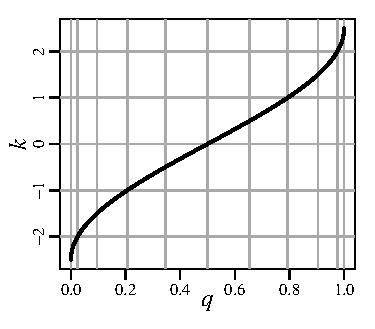
\includegraphics[width=2.5in]{figures/k-q-plot.pdf} 
   \caption{The scale function translates the quantile $q$ to the scale factor $k$ in order to give variable size steps in $q$. Limiting cluster sizes allows better accuracy near $q=0$ or $q=1$. }
   \label{fig:k-q-plot}
\end{figure}
\begin{figure}[p] %  figure placement: here, top, bottom, or page
   \centering
   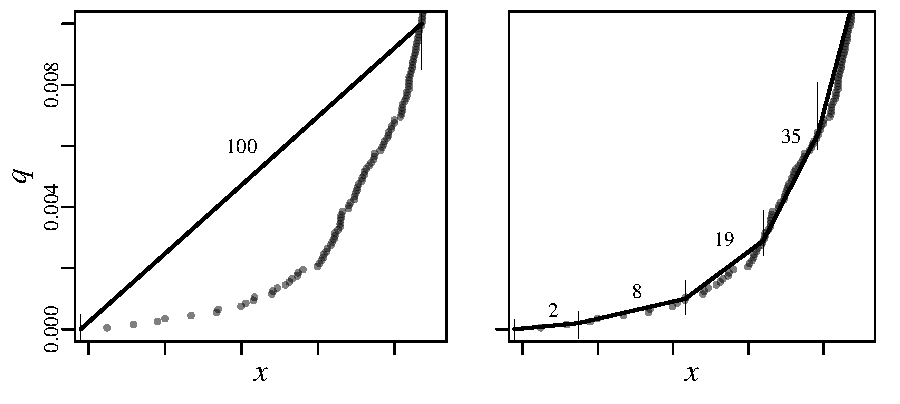
\includegraphics[height=2.in, clip]{figures/linear-interpolation.pdf} 
   \caption{The left panel shows linear interpolation of the cumulative distribution function near $q=0$ with $100$ equal sized bins applied to $10,000$ data points sampled from an exponential distribution. The right panel shows the same interpolation with variable size bins as given by a strongly ordered $t$-digest with $\delta=100$. The numbers above the data points represent the number of points in each bin. }
   \label{fig:linear-interpolation}
\end{figure}
\begin{figure}[p] %  figure placement: here, top, bottom, or page
   \centering
   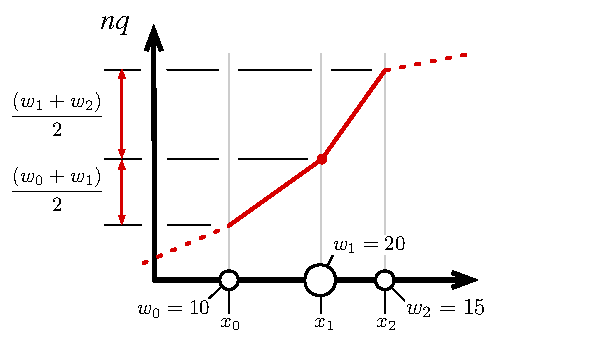
\includegraphics[width=3in]{figures/interpolation.pdf} 
   \caption{Interpolation of the empirical cumulative distribution function between centroids of clusters with more than one sample is done by assuming half of the points for each centroid are to the left of the centroid and half are to the right. }
   \label{fig:interpolation}
\end{figure}

\begin{figure}[p] %  figure placement: here, top, bottom, or page
   \centering
   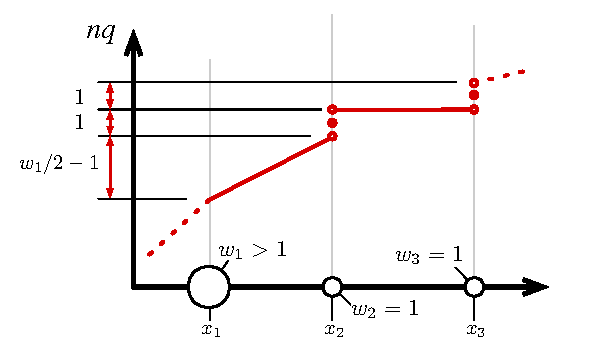
\includegraphics[width=3in]{figures/singleton.pdf} 
   \caption{Clusters with a single sample are handled specially. Adjacent to a normal cluster, as is the case between $x_1$ and $x_2$, interpolation is done assuming $w_1/2$ samples occur between $x_1$ and $x_2$, and the single sample at $x_2$. That single sample causes the cumulative distribution to step to the mid-point of the individual sample at $x_2$. Between singleton clusters $x_2$ and $x_3$, the cumulative distribution is given a constant value until it steps again at $x_3$.}
   \label{fig:singletons}
\end{figure}
\begin{figure}[p] %  figure placement: here, top, bottom, or page
   \centering
   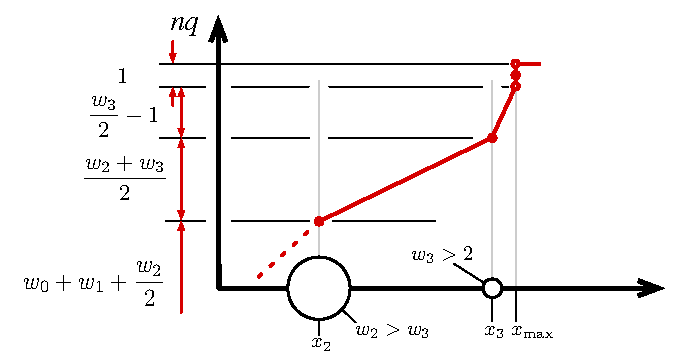
\includegraphics[width=3in]{figures/endpoint.pdf} 
   \caption{For the last clusters, if the cluster weight is greater than $2$, we can use the fact that a singleton must occur at $x_{\mathrm {min}}$ or $x_{\mathrm {max}}$ to improve interpolation accuracy. The first cluster is handled by reversing these steps.}
   \label{fig:endpoint}
\end{figure}
\begin{figure}[p] %  figure placement: here, top, bottom, or page
   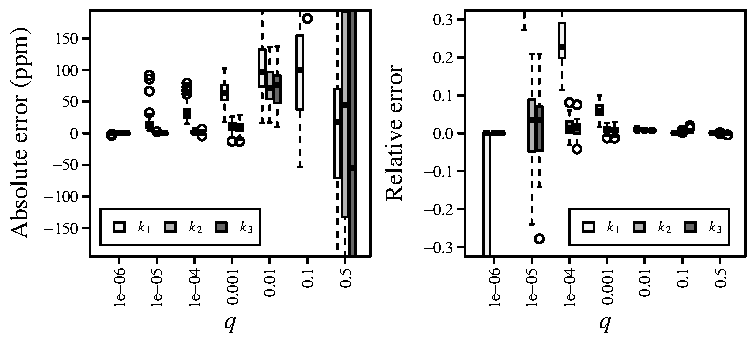
\includegraphics[width=5.5in]{figures/relative-error.pdf} 
   \caption{The left panel shows absolute error in parts per million of estimations of quantile with $\delta = 100$ for scale functions $k_1$, $k_2$ and $k_3$. Errors are computed by taking $10^6$ samples from a uniform distribution and comparing estimates from a $t$-digest against exact quantiles computed from the original samples. This was repeated 50 times to get a sense of variability. The left panel shows absolute error in parts per million and the right panel shows relative error.}
   \label{fig:by-scale}
\end{figure}

\begin{figure}[p] %  figure placement: here, top, bottom, or page
   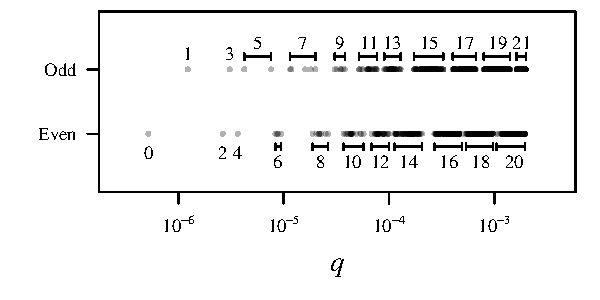
\includegraphics[width=4.5in]{figures/cluster-spread.pdf} 
   \caption{The first few clusters in a typical $t$-digest show that while the digest is not strictly ordered, only adjacent clusters overlap. This plot shows roughly the first 20 clusters of the digest with even-numbered clusters below and odd-numbered ones above. Note how odd clusters overlap with adjacent even clusters, but never with adjacent odd clusters. This corresponds to weak ordering with $\Delta=1$  }
   \label{fig:cluster-spread}
\end{figure}


\begin{figure}[p] %  figure placement: here, top, bottom, or page
   \centering
   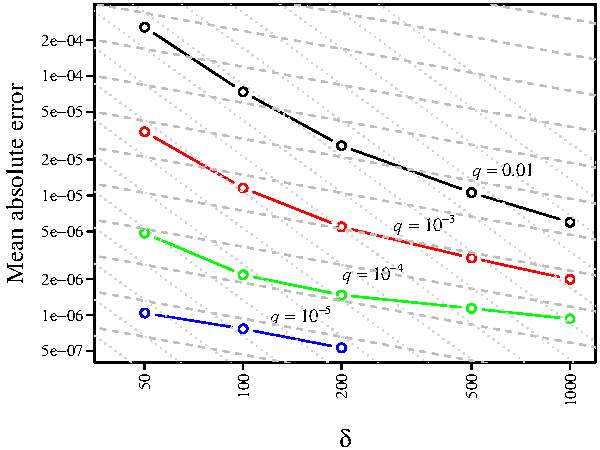
\includegraphics[width=4in]{figures/error-vs-compression.pdf} 
   \caption{The scaling of quantile estimation for various values of compression factor $\delta$ and $q$. 
   The general pattern is that absolute error scales like $1/\delta^2$ for small values of $\delta$ and like $1/\sqrt{\delta}$ for values larger than some cutoff. The cutoff is higher for larger values of $q$ (roughly 500 for $q=0.01$ but only 100 for $q=10^{-5}$). The grey dashed lines provide a reference for $1/\sqrt{\delta}$ scaling, the dotted grey lines show $1/\delta^2$.   At $q=10^{-5}$ error goes to zero for values $\delta > 200$ and cannot be shown on a log scale. The same happens for $q=10^{-6}$ except error is zero for all values of $\delta$. The data shown here are for $k_2$, but the results for $k_3$ are nearly indistinguishable.}
   \label{fig:accuracy-scaling}
\end{figure}



\begin{figure}[p] %  figure placement: here, top, bottom, or page
   \centering
   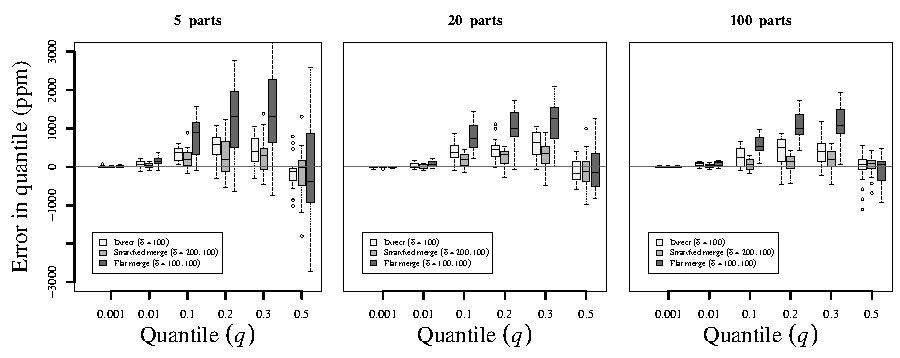
\includegraphics[width=5.5in]{figures/merge.pdf} 
   \caption{Accuracy of a $t$-digest accumulated directly is nearly the same as when the digest is computed by combining digests from 5, 20 or 100 equal sized paritions of the data.  All panels were computed by 20 repetitions of aggregating 1,000,000 values. }
   \label{fig:merge}
\end{figure}
\begin{figure}[p] %  figure placement: here, top, bottom, or page
   \centering
   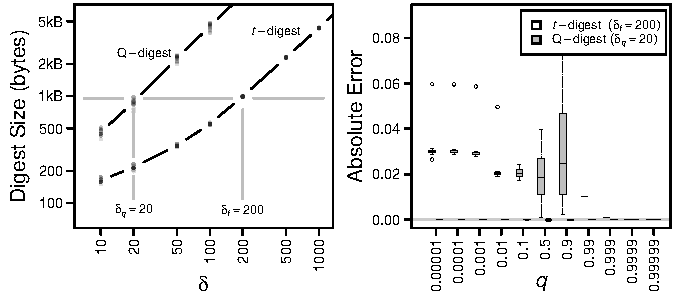
\includegraphics[width=4.5in]{figures/qd-sizes.pdf} 
   \caption{The left panel shows the size of a serialized Q-digest and $t$-digest versus compression parameter $\delta$ for 100,000 uniformly distributed samples. Trials were repeated 20 times. The left panel shows how compression parameters $\delta_q$ and $\delta_t$ are chosen to control digest size to approximately 1k byte. The right panel shows absolute error for various values of $q$.  With this vertical scale, $t$-digest errors are only barely distinguishable from zero near the median.  }
   \label{fig:qd-comparison}
\end{figure}
%\subsection{}
\bibliographystyle{alpha}
\bibliography{refs}{}

\end{document}  
